
%% bare_jrnl_compsoc.tex
%% V1.4
%% 2012/12/27
%% by Michael Shell
%% See:
%% http://www.michaelshell.org/
%% for current contact information.
%%
%% This is a skeleton file demonstrating the use of IEEEtran.cls
%% (requires IEEEtran.cls version 1.8 or later) with an IEEE Computer
%% Society journal paper.
%%
%% Support sites:
%% http://www.michaelshell.org/tex/ieeetran/
%% http://www.ctan.org/tex-archive/macros/latex/contrib/IEEEtran/
%% and
%% http://www.ieee.org/

%%*************************************************************************
%% Legal Notice:
%% This code is offered as-is without any warranty either expressed or
%% implied; without even the implied warranty of MERCHANTABILITY or
%% FITNESS FOR A PARTICULAR PURPOSE! 
%% User assumes all risk.
%% In no event shall IEEE or any contributor to this code be liable for
%% any damages or losses, including, but not limited to, incidental,
%% consequential, or any other damages, resulting from the use or misuse
%% of any information contained here.
%%
%% All comments are the opinions of their respective authors and are not
%% necessarily endorsed by the IEEE.
%%
%% This work is distributed under the LaTeX Project Public License (LPPL)
%% ( http://www.latex-project.org/ ) version 1.3, and may be freely used,
%% distributed and modified. A copy of the LPPL, version 1.3, is included
%% in the base LaTeX documentation of all distributions of LaTeX released
%% 2003/12/01 or later.
%% Retain all contribution notices and credits.
%% ** Modified files should be clearly indicated as such, including  **
%% ** renaming them and changing author support contact information. **
%%
%% File list of work: IEEEtran.cls, IEEEtran_HOWTO.pdf, bare_adv.tex,
%%                    bare_conf.tex, bare_jrnl.tex, bare_jrnl_compsoc.tex,
%%                    bare_jrnl_transmag.tex
%%*************************************************************************

% *** Authors should verify (and, if needed, correct) their LaTeX system  ***
% *** with the testflow diagnostic prior to trusting their LaTeX platform ***
% *** with production work. IEEE's font choices can trigger bugs that do  ***
% *** not appear when using other class files.                            ***
% The testflow support page is at:
% http://www.michaelshell.org/tex/testflow/




% Note that the a4paper option is mainly intended so that authors in
% countries using A4 can easily print to A4 and see how their papers will
% look in print - the typesetting of the document will not typically be
% affected with changes in paper size (but the bottom and side margins will).
% Use the testflow package mentioned above to verify correct handling of
% both paper sizes by the user's LaTeX system.
%
% Also note that the "draftcls" or "draftclsnofoot", not "draft", option
% should be used if it is desired that the figures are to be displayed in
% draft mode.
%
% The Computer Society usually requires 12pt for submissions.
%
\documentclass[12pt,journal,compsoc]{IEEEtran}
%
% If IEEEtran.cls has not been installed into the LaTeX system files,
% manually specify the path to it like:
% \documentclass[12pt,journal,compsoc]{../sty/IEEEtran}





% Some very useful LaTeX packages include:
% (uncomment the ones you want to load)


% *** MISC UTILITY PACKAGES ***
%
%\usepackage{ifpdf}
% Heiko Oberdiek's ifpdf.sty is very useful if you need conditional
% compilation based on whether the output is pdf or dvi.
% usage:
% \ifpdf
%   % pdf code
% \else
%   % dvi code
% \fi
% The latest version of ifpdf.sty can be obtained from:
% http://www.ctan.org/tex-archive/macros/latex/contrib/oberdiek/
% Also, note that IEEEtran.cls V1.7 and later provides a builtin
% \ifCLASSINFOpdf conditional that works the same way.
% When switching from latex to pdflatex and vice-versa, the compiler may
% have to be run twice to clear warning/error messages.






% *** CITATION PACKAGES ***
%
\ifCLASSOPTIONcompsoc
  % IEEE Computer Society needs nocompress option
  % requires cite.sty v4.0 or later (November 2003)
   \usepackage[nocompress]{cite}
\else
  % normal IEEE
   \usepackage{cite}
\fi
% cite.sty was written by Donald Arseneau
% V1.6 and later of IEEEtran pre-defines the format of the cite.sty package
% \cite{} output to follow that of IEEE. Loading the cite package will
% result in citation numbers being automatically sorted and properly
% "compressed/ranged". e.g., [1], [9], [2], [7], [5], [6] without using
% cite.sty will become [1], [2], [5]--[7], [9] using cite.sty. cite.sty's
% \cite will automatically add leading space, if needed. Use cite.sty's
% noadjust option (cite.sty V3.8 and later) if you want to turn this off
% such as if a citation ever needs to be enclosed in parenthesis.
% cite.sty is already installed on most LaTeX systems. Be sure and use
% version 4.0 (2003-05-27) and later if using hyperref.sty. cite.sty does
% not currently provide for hyperlinked citations.
% The latest version can be obtained at:
% http://www.ctan.org/tex-archive/macros/latex/contrib/cite/
% The documentation is contained in the cite.sty file itself.
%
% Note that some packages require special options to format as the Computer
% Society requires. In particular, Computer Society  papers do not use
% compressed citation ranges as is done in typical IEEE papers
% (e.g., [1]-[4]). Instead, they list every citation separately in order
% (e.g., [1], [2], [3], [4]). To get the latter we need to load the cite
% package with the nocompress option which is supported by cite.sty v4.0
% and later. Note also the use of a CLASSOPTION conditional provided by
% IEEEtran.cls V1.7 and later.





% *** GRAPHICS RELATED PACKAGES ***
%
\ifCLASSINFOpdf
  % \usepackage[pdftex]{graphicx}
  % declare the path(s) where your graphic files are
  % \graphicspath{{../pdf/}{../jpeg/}}
  % and their extensions so you won't have to specify these with
  % every instance of \includegraphics
  % \DeclareGraphicsExtensions{.pdf,.jpeg,.png}
\else
  % or other class option (dvipsone, dvipdf, if not using dvips). graphicx
  % will default to the driver specified in the system graphics.cfg if no
  % driver is specified.
  % \usepackage[dvips]{graphicx}
  % declare the path(s) where your graphic files are
  % \graphicspath{{../eps/}}
  % and their extensions so you won't have to specify these with
  % every instance of \includegraphics
  % \DeclareGraphicsExtensions{.eps}
\fi
% graphicx was written by David Carlisle and Sebastian Rahtz. It is
% required if you want graphics, photos, etc. graphicx.sty is already
% installed on most LaTeX systems. The latest version and documentation
% can be obtained at: 
% http://www.ctan.org/tex-archive/macros/latex/required/graphics/
% Another good source of documentation is "Using Imported Graphics in
% LaTeX2e" by Keith Reckdahl which can be found at:
% http://www.ctan.org/tex-archive/info/epslatex/
%
% latex, and pdflatex in dvi mode, support graphics in encapsulated
% postscript (.eps) format. pdflatex in pdf mode supports graphics
% in .pdf, .jpeg, .png and .mps (metapost) formats. Users should ensure
% that all non-photo figures use a vector format (.eps, .pdf, .mps) and
% not a bitmapped formats (.jpeg, .png). IEEE frowns on bitmapped formats
% which can result in "jaggedy"/blurry rendering of lines and letters as
% well as large increases in file sizes.
%
% You can find documentation about the pdfTeX application at:
% http://www.tug.org/applications/pdftex


\usepackage{enumerate}
\usepackage{graphicx}

\usepackage{listings}  % produces code listings for all languages
\usepackage{fancyvrb}  % a better verbatim environment
\usepackage{enumitem}  % control enumerate, itemize environments
\usepackage{etoolbox}  % add to existing environments
\usepackage{rotating}  % landscape figures

\usepackage{amsthm}    % mathematics packages
\usepackage{amsmath}
\usepackage{amssymb}


% ACL2 command for embedded text
\renewcommand{\a}[1]{{\tt\small #1}}



% ACL2 block environment
\lstnewenvironment{acl2-lst}
{\lstset{
    language=LISP,
    basicstyle=\ttfamily\small,
    breaklines=true,
    columns=fixed,
    basewidth=.5em,
    xleftmargin=.25in,
    escapeinside={&[}{]&},
    aboveskip=12pt,
    belowskip=12pt,
    lineskip=-1pt,
    frame=none,
    mathescape,
    numbers=left
  }}
{}

% Modifies ACL2 environment to prevent page breaking
%\BeforeBeginEnvironment{acl2-lst}{\par\noindent\begin{minipage}[!h]{\textwidth}}
%\AfterEndEnvironment{acl2-lst}{\end{minipage}}


% *** MATH PACKAGES ***
%
% A popular package from the American Mathematical Society that provides
% many useful and powerful commands for dealing with mathematics. If using
% it, be sure to load this package with the cmex10 option to ensure that
% only type 1 fonts will utilized at all point sizes. Without this option,
% it is possible that some math symbols, particularly those within
% footnotes, will be rendered in bitmap form which will result in a
% document that can not be IEEE Xplore compliant!
%
% Also, note that the amsmath package sets \interdisplaylinepenalty to 10000
% thus preventing page breaks from occurring within multiline equations. Use:
%\interdisplaylinepenalty=2500
% after loading amsmath to restore such page breaks as IEEEtran.cls normally
% does. amsmath.sty is already installed on most LaTeX systems. The latest
% version and documentation can be obtained at:
% http://www.ctan.org/tex-archive/macros/latex/required/amslatex/math/





% *** SPECIALIZED LIST PACKAGES ***
%
%\usepackage{algorithmic}
% algorithmic.sty was written by Peter Williams and Rogerio Brito.
% This package provides an algorithmic environment fo describing algorithms.
% You can use the algorithmic environment in-text or within a figure
% environment to provide for a floating algorithm. Do NOT use the algorithm
% floating environment provided by algorithm.sty (by the same authors) or
% algorithm2e.sty (by Christophe Fiorio) as IEEE does not use dedicated
% algorithm float types and packages that provide these will not provide
% correct IEEE style captions. The latest version and documentation of
% algorithmic.sty can be obtained at:
% http://www.ctan.org/tex-archive/macros/latex/contrib/algorithms/
% There is also a support site at:
% http://algorithms.berlios.de/index.html
% Also of interest may be the (relatively newer and more customizable)
% algorithmicx.sty package by Szasz Janos:
% http://www.ctan.org/tex-archive/macros/latex/contrib/algorithmicx/




% *** ALIGNMENT PACKAGES ***
%
%\usepackage{array}
% Frank Mittelbach's and David Carlisle's array.sty patches and improves
% the standard LaTeX2e array and tabular environments to provide better
% appearance and additional user controls. As the default LaTeX2e table
% generation code is lacking to the point of almost being broken with
% respect to the quality of the end results, all users are strongly
% advised to use an enhanced (at the very least that provided by array.sty)
% set of table tools. array.sty is already installed on most systems. The
% latest version and documentation can be obtained at:
% http://www.ctan.org/tex-archive/macros/latex/required/tools/


% IEEEtran contains the IEEEeqnarray family of commands that can be used to
% generate multiline equations as well as matrices, tables, etc., of high
% quality.




% *** SUBFIGURE PACKAGES ***
%\ifCLASSOPTIONcompsoc
%  \usepackage[caption=false,font=normalsize,labelfont=sf,textfont=sf]{subfig}
%\else
%  \usepackage[caption=false,font=footnotesize]{subfig}
%\fi
% subfig.sty, written by Steven Douglas Cochran, is the modern replacement
% for subfigure.sty, the latter of which is no longer maintained and is
% incompatible with some LaTeX packages including fixltx2e. However,
% subfig.sty requires and automatically loads Axel Sommerfeldt's caption.sty
% which will override IEEEtran.cls' handling of captions and this will result
% in non-IEEE style figure/table captions. To prevent this problem, be sure
% and invoke subfig.sty's "caption=false" package option (available since
% subfig.sty version 1.3, 2005/06/28) as this is will preserve IEEEtran.cls
% handling of captions.
% Note that the Computer Society format requires a larger sans serif font
% than the serif footnote size font used in traditional IEEE formatting
% and thus the need to invoke different subfig.sty package options depending
% on whether compsoc mode has been enabled.
%
% The latest version and documentation of subfig.sty can be obtained at:
% http://www.ctan.org/tex-archive/macros/latex/contrib/subfig/




% *** FLOAT PACKAGES ***
%
%\usepackage{fixltx2e}
% fixltx2e, the successor to the earlier fix2col.sty, was written by
% Frank Mittelbach and David Carlisle. This package corrects a few problems
% in the LaTeX2e kernel, the most notable of which is that in current
% LaTeX2e releases, the ordering of single and double column floats is not
% guaranteed to be preserved. Thus, an unpatched LaTeX2e can allow a
% single column figure to be placed prior to an earlier double column
% figure. The latest version and documentation can be found at:
% http://www.ctan.org/tex-archive/macros/latex/base/


%\usepackage{stfloats}
% stfloats.sty was written by Sigitas Tolusis. This package gives LaTeX2e
% the ability to do double column floats at the bottom of the page as well
% as the top. (e.g., "\begin{figure*}[!b]" is not normally possible in
% LaTeX2e). It also provides a command:
%\fnbelowfloat
% to enable the placement of footnotes below bottom floats (the standard
% LaTeX2e kernel puts them above bottom floats). This is an invasive package
% which rewrites many portions of the LaTeX2e float routines. It may not work
% with other packages that modify the LaTeX2e float routines. The latest
% version and documentation can be obtained at:
% http://www.ctan.org/tex-archive/macros/latex/contrib/sttools/
% Do not use the stfloats baselinefloat ability as IEEE does not allow
% \baselineskip to stretch. Authors submitting work to the IEEE should note
% that IEEE rarely uses double column equations and that authors should try
% to avoid such use. Do not be tempted to use the cuted.sty or midfloat.sty
% packages (also by Sigitas Tolusis) as IEEE does not format its papers in
% such ways.
% Do not attempt to use stfloats with fixltx2e as they are incompatible.
% Instead, use Morten Hogholm'a dblfloatfix which combines the features
% of both fixltx2e and stfloats:
%
% \usepackage{dblfloatfix}
% The latest version can be found at:
% http://www.ctan.org/tex-archive/macros/latex/contrib/dblfloatfix/




%\ifCLASSOPTIONcaptionsoff
%  \usepackage[nomarkers]{endfloat}
% \let\MYoriglatexcaption\caption
% \renewcommand{\caption}[2][\relax]{\MYoriglatexcaption[#2]{#2}}
%\fi
% endfloat.sty was written by James Darrell McCauley, Jeff Goldberg and 
% Axel Sommerfeldt. This package may be useful when used in conjunction with 
% IEEEtran.cls'  captionsoff option. Some IEEE journals/societies require that
% submissions have lists of figures/tables at the end of the paper and that
% figures/tables without any captions are placed on a page by themselves at
% the end of the document. If needed, the draftcls IEEEtran class option or
% \CLASSINPUTbaselinestretch interface can be used to increase the line
% spacing as well. Be sure and use the nomarkers option of endfloat to
% prevent endfloat from "marking" where the figures would have been placed
% in the text. The two hack lines of code above are a slight modification of
% that suggested by in the endfloat docs (section 8.4.1) to ensure that
% the full captions always appear in the list of figures/tables - even if
% the user used the short optional argument of \caption[]{}.
% IEEE papers do not typically make use of \caption[]'s optional argument,
% so this should not be an issue. A similar trick can be used to disable
% captions of packages such as subfig.sty that lack options to turn off
% the subcaptions:
% For subfig.sty:
% \let\MYorigsubfloat\subfloat
% \renewcommand{\subfloat}[2][\relax]{\MYorigsubfloat[]{#2}}
% However, the above trick will not work if both optional arguments of
% the \subfloat command are used. Furthermore, there needs to be a
% description of each subfigure *somewhere* and endfloat does not add
% subfigure captions to its list of figures. Thus, the best approach is to
% avoid the use of subfigure captions (many IEEE journals avoid them anyway)
% and instead reference/explain all the subfigures within the main caption.
% The latest version of endfloat.sty and its documentation can obtained at:
% http://www.ctan.org/tex-archive/macros/latex/contrib/endfloat/
%
% The IEEEtran \ifCLASSOPTIONcaptionsoff conditional can also be used
% later in the document, say, to conditionally put the References on a 
% page by themselves.




% *** PDF, URL AND HYPERLINK PACKAGES ***
%
%\usepackage{url}
% url.sty was written by Donald Arseneau. It provides better support for
% handling and breaking URLs. url.sty is already installed on most LaTeX
% systems. The latest version and documentation can be obtained at:
% http://www.ctan.org/tex-archive/macros/latex/contrib/url/
% Basically, \url{my_url_here}.





% *** Do not adjust lengths that control margins, column widths, etc. ***
% *** Do not use packages that alter fonts (such as pslatex).         ***
% There should be no need to do such things with IEEEtran.cls V1.6 and later.
% (Unless specifically asked to do so by the journal or conference you plan
% to submit to, of course. )


% correct bad hyphenation here
\hyphenation{op-tical net-works semi-conduc-tor}


\begin{document}
%
% paper title
% can use linebreaks \\ within to get better formatting as desired
% Do not put math or special symbols in the title.
\title{Using ACL2 to Prove the Correctness of Lowering Operators when $J=l+s$}
%
%
% author names and IEEE memberships
% note positions of commas and nonbreaking spaces ( ~ ) LaTeX will not break
% a structure at a ~ so this keeps an author's name from being broken across
% two lines.
% use \thanks{} to gain access to the first footnote area
% a separate \thanks must be used for each paragraph as LaTeX2e's \thanks
% was not built to handle multiple paragraphs
%
%
%\IEEEcompsocitemizethanks is a special \thanks that produces the bulleted
% lists the Computer Society journals use for "first footnote" author
% affiliations. Use \IEEEcompsocthanksitem which works much like \item
% for each affiliation group. When not in compsoc mode,
% \IEEEcompsocitemizethanks becomes like \thanks and
% \IEEEcompsocthanksitem becomes a line break with idention. This
% facilitates dual compilation, although admittedly the differences in the
% desired content of \author between the different types of papers makes a
% one-size-fits-all approach a daunting prospect. For instance, compsoc 
% journal papers have the author affiliations above the "Manuscript
% received ..."  text while in non-compsoc journals this is reversed. Sigh.

\author{Chen,~Xiaohui\\
	Department of Computer Science\\
	The University of Texas at Austin% <-this % stops a space 
	}

% note the % following the last \IEEEmembership and also \thanks - 
% these prevent an unwanted space from occurring between the last author name
% and the end of the author line. i.e., if you had this:
% 
% \author{....lastname \thanks{...} \thanks{...} }
%                     ^------------^------------^----Do not want these spaces!
%
% a space would be appended to the last name and could cause every name on that
% line to be shifted left slightly. This is one of those "LaTeX things". For
% instance, "\textbf{A} \textbf{B}" will typeset as "A B" not "AB". To get
% "AB" then you have to do: "\textbf{A}\textbf{B}"
% \thanks is no different in this regard, so shield the last } of each \thanks
% that ends a line with a % and do not let a space in before the next \thanks.
% Spaces after \IEEEmembership other than the last one are OK (and needed) as
% you are supposed to have spaces between the names. For what it is worth,
% this is a minor point as most people would not even notice if the said evil
% space somehow managed to creep in.



% The paper headers
\markboth{Spring 2015 CS 389R Project Written Report}%
{Prove the Correctness of Lowering Operators}
% The only time the second header will appear is for the odd numbered pages
% after the title page when using the twoside option.
% 
% *** Note that you probably will NOT want to include the author's ***
% *** name in the headers of peer review papers.                   ***
% You can use \ifCLASSOPTIONpeerreview for conditional compilation here if
% you desire.



% The publisher's ID mark at the bottom of the page is less important with
% Computer Society journal papers as those publications place the marks
% outside of the main text columns and, therefore, unlike regular IEEE
% journals, the available text space is not reduced by their presence.
% If you want to put a publisher's ID mark on the page you can do it like
% this:
%\IEEEpubid{0000--0000/00\$00.00~\copyright~2012 IEEE}
% or like this to get the Computer Society new two part style.
%\IEEEpubid{\makebox[\columnwidth]{\hfill 0000--0000/00/\$00.00~\copyright~2012 IEEE}%
%\hspace{\columnsep}\makebox[\columnwidth]{Published by the IEEE Computer Society\hfill}}
% Remember, if you use this you must call \IEEEpubidadjcol in the second
% column for its text to clear the IEEEpubid mark (Computer Society jorunal
% papers don't need this extra clearance.)



% use for special paper notices
%\IEEEspecialpapernotice{(Invited Paper)}



% for Computer Society papers, we must declare the abstract and index terms
% PRIOR to the title within the \IEEEtitleabstractindextext IEEEtran
% command as these need to go into the title area created by \maketitle.
% As a general rule, do not put math, special symbols or citations
% in the abstract or keywords.
\IEEEtitleabstractindextext{%
\begin{abstract}
Lowering Operators can be used to calcualte the Clebsch-Gordan coefficients in quantum coupled states. In this paper I am going to use ACL2 to verify that when the lowering operators operates on some initial quantum states, the coefficients match the Clebsch-Gordan coefficients and satisfy the probability rules. In addition, possible future research is proposed.
\end{abstract}

% Note that keywords are not normally used for peerreview papers.
\begin{IEEEkeywords}
Quantum coupling, Clebsch-Gordan coefficient, angular momentum, ACL2, recursion and induction
\end{IEEEkeywords}}


% make the title area
\maketitle


% To allow for easy dual compilation without having to reenter the
% abstract/keywords data, the \IEEEtitleabstractindextext text will
% not be used in maketitle, but will appear (i.e., to be "transported")
% here as \IEEEdisplaynontitleabstractindextext when the compsoc 
% or transmag modes are not selected <OR> if conference mode is selected 
% - because all conference papers position the abstract like regular
% papers do.
\IEEEdisplaynontitleabstractindextext
% \IEEEdisplaynontitleabstractindextext has no effect when using
% compsoc or transmag under a non-conference mode.



% For peer review papers, you can put extra information on the cover
% page as needed:
% \ifCLASSOPTIONpeerreview
% \begin{center} \bfseries EDICS Category: 3-BBND \end{center}
% \fi
%
% For peerreview papers, this IEEEtran command inserts a page break and
% creates the second title. It will be ignored for other modes.
\IEEEpeerreviewmaketitle



\section{Introduction}
% Computer Society journal papers do something a tad strange with the very
% first section heading (almost always called "Introduction"). They place it
% ABOVE the main text! IEEEtran.cls currently does not do this for you.
% However, You can achieve this effect by making LaTeX jump through some
% hoops via something like:
%
%\ifCLASSOPTIONcompsoc
%  \noindent\raisebox{2\baselineskip}[0pt][0pt]%
%  {\parbox{\columnwidth}{\section{Introduction}\label{sec:introduction}%
%  \global\everypar=\everypar}}%
%  \vspace{-1\baselineskip}\vspace{-\parskip}\par
%\else
%  \section{Introduction}\label{sec:introduction}\par
%\fi
%
% Admittedly, this is a hack and may well be fragile, but seems to do the
% trick for me. Note the need to keep any \label that may be used right
% after \section in the above as the hack puts \section within a raised box.



% The very first letter is a 2 line initial drop letter followed
% by the rest of the first word in caps (small caps for compsoc).
% 
% form to use if the first word consists of a single letter:
% \IEEEPARstart{A}{demo} file is ....
% 
% form to use if you need the single drop letter followed by
% normal text (unknown if ever used by IEEE):
% \IEEEPARstart{A}{}demo file is ....
% 
% Some journals put the first two words in caps:
% \IEEEPARstart{T}{his demo} file is ....
% 
% Here we have the typical use of a "T" for an initial drop letter
% and "HIS" in caps to complete the first word.
\IEEEPARstart{C}{lebsch-Gordan} coefficients are mathematical symbol used to integrate products of three spherical harmonics \cite{clebsch}. 
Sphereical harmonics are some functions defined on the surface of a sphere. In quantum phycis, they are used to represent the boundaries of the particles. A sphererical harmonic function is defined as $Y_{l}^{m_l}(\theta,\phi)$ where $l$ and $m_l$ are quantum numbers (details described later).
Clebsch-Gordan coefficients represent the probability of the particles in those coupled states. According to fundamental rules of probability, the sum of all probabilities of the coupled states in a certain joint state equals to 1. In this paper, I am using ACL2 to verfy such property is still valid when lowering operators are operated on certain quantum states. 

Normally, for two-particle systems, we can easily fiure out the total angular momenta $\vec{J}$ and the z-component of $\vec{J}$, $\vec{m_{J}}$. However, we could not know the angular momentum of each particle $\vec{l}$ and $\vec{s}$. Clebsch-Gordan coefficients can give the probabilties of the particles in each possible set of angular momenta. Therefore Clebsch-Gordan coefficients are very important in determining the angular momenta of two particle systems.

The handproofs of the correctness of calculating Clebsch-Gordan coefficients using lowering operators is lengthy and tedious. Therefore, if ACL2 theorem prover can prove the correctness, it can save a large amount of work. In addition, ACL2 theorem prover can verify the correctness of the handproofs.

First of all, this paper provides the background knowledge. It introduces the concept of quantum coupling, Clebsch Gordan coefficient, and lowering operators.

Then this paper will introduce ACL2, which is a programming language capable of modeling computer systems as well as proving properties of those systems. The quantum-state model described in this paper is implemented in ACL2 and the properties and main theorems are proved in ACL2.

After introducing my model, this paper will discuss how j-states, coupled states and quantuam states are implemented. Also, properties of those models will be discussed and procedures in proving those properties will be introduced.

After discussing my models, this paper will discuss how lowering operators operate on initial states and verify if the output satisfies Clebsch-Gordan coefficients and probability rules.

Finally, possible future research areas and possible improvements are discussed in this paper.

% You must have at least 2 lines in the paragraph with the drop letter
% (should never be an issue)

\section{Background Knowledge}

Some background knowledge is necessary in order to fully understand this paper.

\subsection{Angular Momemtum}

In this paper, we have two angular momenta. The first angular momentum is denoted as $\vec{l}$ and the second momemtum is denoted as $\vec{s}$. Their projections onto the z-axis are denoted as $\vec{m_l}$ and $\vec{m_s}$ respectively. 

Therefore, $l$, $m_l$, $s$, and $m_s$ are quantum numbers. Here $l$ and $s$ represent the two angular momenta, while $m_l$ and $m_s$ represent the z-compoment of $l$ and $s$. In quantum physics, those quantum numbers satisfy the following conditions:

\begin{enumerate}

\item $l>0$ and $s>0$

\item $l$ is either an integer or a half-integer (with denominator 2). Same for $s$

\item $m_l= -l, -l+1, \ldots, l$, $m_s= -s, -s+1, \ldots, s$

\item If $l$ is an integer, then $m_l$ is an integer. Otherwise $m_l$ is a half-integer. Same for $s$ and $m_s$

\end{enumerate}

\begin{figure}

\centering
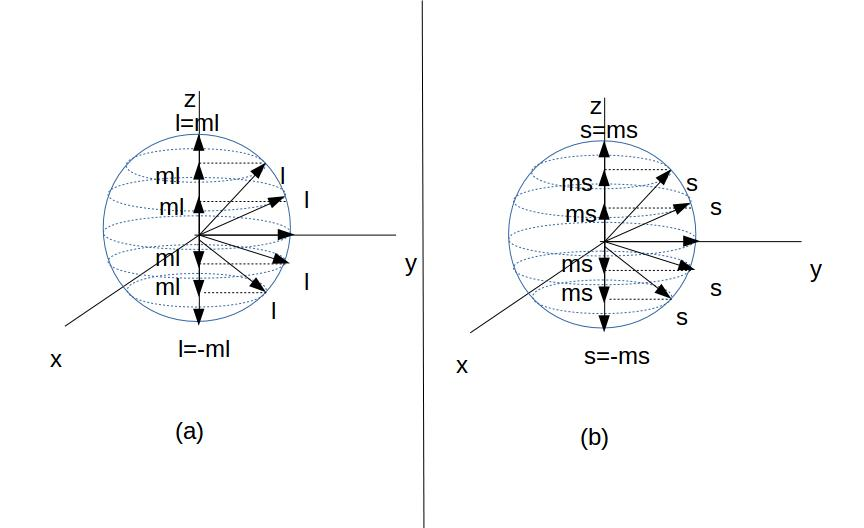
\includegraphics[width=3.8in]{angular}
\caption{The graphical representation of $l$, $m_l$, $s$, and $m_s$. The vectors which has tips on the circle are $\vec{l}$ and $\vec{s}$ recpectively. The vectors on z-axis are $\vec{m_l}$ and $\vec{m_s}$ respectively. Special cases are $|\vec{l}| = |\vec{m_l}|$ and $|\vec{s}|= |\vec{m_s}|$.}
\label{angular}

\end{figure}

The graphical representation of $\vec{l}$, $\vec{s}$, $\vec{m_l}$ and $\vec{m_s}$ is shown in Figure \ref{angular}. 

\begin{figure}

\centering
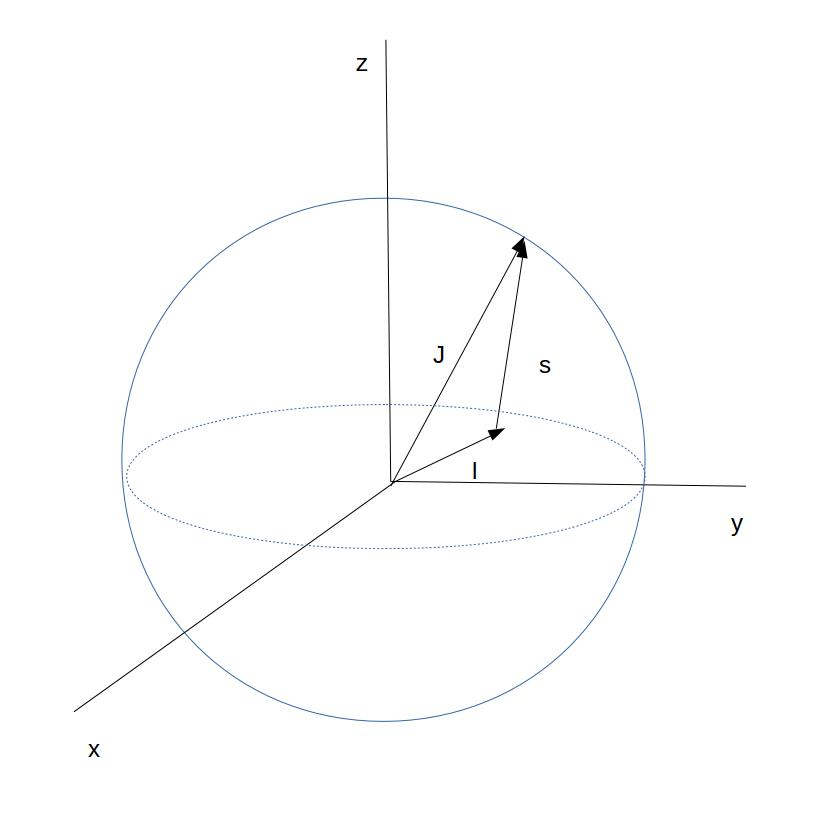
\includegraphics[width=3.8in]{coordinate}
\caption{The graphical representation of $\vec{J}$. Here $\vec{J}$ is the total angular momentum.}
\label{coordinate}

\end{figure}

In this paper, $\vec{J}$ is defined as $\vec{J} = \vec{l} +\vec{s}$. The projection of $\vec{J}$ onto z-axis, $\vec{m_J}$, is therefore $\vec{m_J} = \vec{m_l}+ \vec{m_s}$. The graphical representation of $\vec{J}$ is shown in Figure \ref{coordinate}.

The quantum numbers $J$ and $m_J$ satisfy the following conditions:


\begin{enumerate}

\item $J \ge 0$

\item $J=|l-s|,|l-s|+1,\ldots, l+s$. However, in this project, we only consider $J=l+s$ for simplisity. In the future, we can expand the conditions and let $J$ equals to other values

\item $J$ is either an integer or a half-integer (with denominator 2)

\item $m_J= -J, -J+1, \ldots, J$

\item If $J$ is an integer, then $m_J$ is an integer. Otherwise $m_J$ is a half-integer

\end{enumerate}

\begin{figure}

\centering
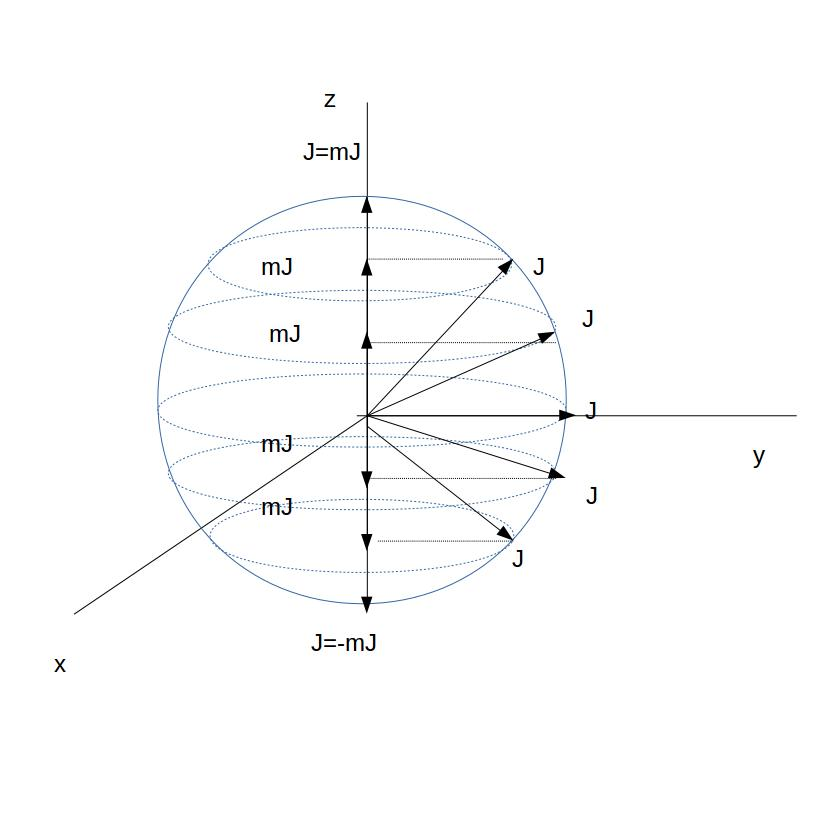
\includegraphics[width=3.8in]{jstate}
\caption{The graphical representation of $\vec{J}$ and $\vec{m_J}$. $\vec{J}$ and $\vec{m_J}$ are very similar than those vectors represented in Figure \ref{angular}.}
\label{jstate}

\end{figure}

Similar to Figure \ref{angular}, $\vec{J}$ and $\vec{m}_J$ are represented in Figure \ref{jstate}.

\subsection{Quantum States}

In quantum physics, quantum states represent the states of quantum system. In this paper, the quantum states are represented in ket-notations. For example $|l,m_l \rangle$  means a particle is in a state such that the particle has quantum numbers $l$ and $m_l$. 

In this paper, $|l,m_l\rangle|s,m_s\rangle$ is a coupled-state, while $|J,m_J\rangle$ is defined as J-state. A quantum state can be represented in the following equation:

\begin{equation}
|J, m_J \rangle = \sum\limits_{m_J = m_l+m_s} c_n |l,m_l\rangle |s,m_s \rangle
\label{clebsch}
\end{equation}


In equation \ref{clebsch}, $|J,m_J \rangle$ is the J-state, which is a state with the quantum numbers of total angular momentum only. In addition, we have $|l,m_l\rangle|s,m_s\rangle$, which is the coupled state with two sets of angular momenta $\vec{l}$ and $\vec{s}$ as quantum numbers. Here, $c_n$ is called the Clebsch-Gordan coefficient. Here $|c_n|^2$ means given the J-state $|J,m_J \rangle$ of a particle, we can know that the particle is in coupled state $|l,m_l\rangle|s,m_s\rangle$ with probability $|c_n|^2$. Therefore, we ca know:

\begin{equation}
\sum\limits_{m_j= m_l+m_s} |c_n|^2 =1
\label{probability}
\end{equation}

My models of quantum states are based on equation \ref{clebsch}. The main theorem to be proved in ACL2 is in fact equation \ref{probability}. More detail will be discussed in next section.

\subsection{Lowering Operators}

Three lowering operators are used in this project: $J_{-}$, $L_{-}$ and $S_{-}$. $J_-$ only operates on the j-state while $L_-$ and $S_-$ only operate on the coupled-state. The lowering operators satisfy the following equations:

\begin{equation}
L_{-} |l,m_l \rangle = \hbar \sqrt{l(l+1)-m_l(m_l - 1)} |l,(m_l - 1) \rangle
\label{l}
\end{equation}

\begin{equation}
S_{-} |s,m_s \rangle = \hbar \sqrt{s(s+1)-m_s(m_s - 1)} |s,(m_s - 1) \rangle
\label{s}
\end{equation}

Since $\vec{J}= \vec{l}+ \vec{s}$, $J_{-}$ obeys the following properties:

\begin{equation}
J_{-}= L_{-} + S_{-}
\label{jsum}
\end{equation}

\begin{equation}
J_{-} |J,m_J \rangle = \hbar \sqrt{J(J+1)-m_J(m_J - 1)} |J,(m_j  - 1) \rangle
\label{j}
\end{equation}

The above equations indicate that the lowering operators do not affect $J$, $l$ and $s$. However, after each operators operating on the quantum states, $m_J$, $m_l$ and $m_l$ are lowered by 1. 

In equation \ref{clebsch}, $J_-$ operates on left-hand-side while $L_-$ and $S_-$ operate on the right-hand-side. A specific example is given below.\\

We have an electron with angular momentum $l=1$ and spin $s=\frac{1}{2}$

Therefore $m_l=-1,0,-1$ and $m_s= \pm \frac{1}{2}$

This means $J=\frac{3}{2}$ and $m_J= -\frac{3}{2}, - \frac{1}{2}, \frac{1}{2}, \frac{3}{2}$

We know that the only possibility of forming $|J,m_J\rangle= |\frac{3}{2},\frac{3}{2}\rangle$ is $|\frac{3}{2}\,\frac{3}{2}\rangle = |1,1\rangle |\frac{1}{2},\frac{1}{2}\rangle $.

Applying the lowering operator on the above equation

\begin{equation}
\begin{aligned}
J_{-}|\frac{3}{2},\frac{3}{2}\rangle =  \hbar \sqrt{\frac{3}{2} \left( \frac{3}{2}+1 \right) -  \frac{3}{2} \left( \frac{3}{2}-1 \right)} \\|\frac{3}{2},\frac{1}{2}\rangle = \sqrt{3} \hbar |\frac{3}{2},\frac{1}{2}\rangle
\end{aligned}
\end{equation}

\begin{equation}
\begin{aligned}
J_{-} |1,1\rangle |\frac{1}{2},\frac{1}{2}\rangle = (L_{-}+ S_{-}) |1,1\rangle |\frac{1}{2},\frac{1}{2}\rangle \\= L_{-}|1,1\rangle |\frac{1}{2},\frac{1}{2}\rangle + |1,1\rangle S_{-} |\frac{1}{2},\frac{1}{2}\rangle \\= \hbar\sqrt{1(1+1)-1(1-1)} |1,0\rangle |\frac{1}{2},\frac{1}{2}\rangle\\ + \hbar \sqrt{\frac{1}{2} \left( \frac{1}{2}+1 \right) -  \frac{1}{2} \left( \frac{1}{2}-1 \right)} |1,1\rangle |\frac{1}{2},-\frac{1}{2}\rangle\\ = \hbar \sqrt{2} |1,0\rangle |\frac{1}{2},\frac{1}{2}\rangle + \hbar |1,1\rangle |\frac{1}{2},-\frac{1}{2}\rangle
\end{aligned}
\end{equation}

\begin{equation}
\begin{aligned}
\sqrt{3} \hbar |\frac{3}{2},\frac{1}{2}\rangle = \hbar \sqrt{2} |1,0\rangle |\frac{1}{2},\frac{1}{2}\rangle + \hbar |1,1\rangle |\frac{1}{2},-\frac{1}{2}\rangle
\end{aligned}
\label{subresult}
\end{equation}

Therefore, we have:

\begin{equation}
\begin{aligned}
|\frac{3}{2},\frac{1}{2}\rangle = \sqrt{\frac{2}{3}} |1,0\rangle |\frac{1}{2},\frac{1}{2}\rangle + \frac{1}{\sqrt{3}} |1,1\rangle |\frac{1}{2},-\frac{1}{2}\rangle
\end{aligned}
\label{result}
\end{equation}

Equation \ref{result} satisfies eqaution \ref{probability}. Therefore the lowering operators given in this expample gives valid Clebsch-Gordan Coefficients.

A general form of equation \ref{subresult} can be expressed as follows, with $\hbar$ eliminated on both sides of the equation:

\begin{equation}
\begin{aligned}
\sqrt{A} |J,m_J\rangle = \sqrt{B}|l_1,m_{l1}\rangle|s_1,m_{s1}\rangle \\+ \sqrt{C}|l_2,m_{l2}\rangle|s_2,m_{s2}\rangle+ \ldots
\end{aligned}
\label{main-model}
\end{equation}

There is one special case when $J=-m_J$, $l=-m_l$ and $s=-m_s$. According to equations \ref{j},\ref{l} and \ref{s}, we can know that both sides of equation \ref{main-model} are 0. 

\subsection{ACL2}

ACL2, which stands for "A Computational Logic for Applicative Common Lisp", is a subset of Lisp. It is both a functional programming language based on Common Lisp and a first-order mathematical theory with induction \cite{acl2}.

In addition, ACL2 has a theorem prover, which can be used to prove the properties of the self-defined models. This project utilizes the power to ACL2 to prove that the lowering operators operating on some spefific quantum states gives the correct Clebsch-Gordan coefficients.

Similar to Common Lisp, a function is of the following form:

\begin{verbatim}
(defun function-name (x)
	...)
\end{verbatim}

In order to certify that the recrusive functions would terminate at some points, the function definitions should all satisfy the conditions mentioned in \cite{acl2}. What valid function definitions mean is not the scope of this paper. 

The theorems in ACL2 are of this form:

\begin{verbatim}
(defthm theorem-name
	...)
\end{verbatim}

When a theorem is complied, ACL2 theorem prover will try to prove the correctness of such theorem using induction. The lemmas and main theorem are proved in this way.

\section{My Model}

My model in this project is of this form:

\begin{acl2-lst}[mathescape]
((A . (j . $m_j$)) .   ;j-state
(B . ((l . $m_l$) . (s . $m_s$)))
(C . ((l . $m_l$) . (s . $m_s$)))
...) ;coupled-state
\end{acl2-lst}

As discussed in section 2.3, when the lowering operators operate on the lowest state. The model becomes:

\begin{acl2-lst}[breaklines=true,mathescape]
(0 . 0) 
;This happens when the lowering operators 
;are operated on the lowest states
\end{acl2-lst}

The model is indeed a pair. The car of the pair is the J-state and the cdr of the pair is a list of coupled-states. Other than the conditions described in previous sections, the model satisfies the following conditions:

\begin{enumerate}

\item $A=B+C+ \ldots$

\item The coefficients should be non-negative

\item In my model, J-state and coupled-states are either both 0 or a pair for a J-state and a list for coupled-states

\end{enumerate}

\subsection{J-State}

\subsubsection{Implementation}

As discussed in the previous section, a J-state should be of the form:

\begin{acl2-lst}
(A . (j . $m_j$))
\end{acl2-lst}

Before the actual implementation of J-state, we have several helper functions:

\begin{acl2-lst}
(defun j-coefficient (x) 
 (car x))

(defun quantum-j (x)
 (car (cdr x)))

(defun quantum-mj (x)
 (cdr (cdr x)))

(defun lower-or-lowest-jstate (x)
  (or (>= (- (quantum-mj x)) (quantum-j x))
     (equal (j-coefficient x) 0)))

(defun half-or-full-integer (x)
  (xor (equal (denominator x) 1)
       (equal (denominator x) 2)))

(defun half-full-match (x y)
  (and (iff (equal (denominator x) 1)
	    (equal (denominator y) 1))
       (iff (equal (denominator x) 2)
	    (equal (denominator y) 2))))

(defun rational-pair (x)
  (if (atom x) 
      nil
      (and (rationalp (car x))
	   (< 0 (car x))
	   (rationalp (cdr x))
	   (natp (- (car x) (abs (cdr x))))
	   (half-or-full-integer (car x))
	   (half-or-full-integer (cdr x))
	   (half-full-match (car x) (cdr x))
	   (<= (abs (cdr x)) (car x)))))
\end{acl2-lst}

Functions j-coefficient, quantum-j and quantum-mj returns the specific values of the coefficient or quantum number. The lower-or-lowest-jstate determines whether the j-state is in the lowest state or invalid state ($J<-m_J$). Function half-or-full-integer checks whether the J-state satisfies condition 3 for the J-state (at the end of section 2.1) while half-full-match checks whether condition 5 is satisfied. Finally, rational-pair determines whether condition 4 is satisfied.

Therefore, the function which checks whether the input is a real J-state is given below: 

\begin{acl2-lst}
(defun true-jstate (a)
  (if (atom a)
      (equal a 0)
      (and (rationalp (car a))
	   (<= 0 (car a))  ;Condition 2
	   (rational-pair (cdr a)))))
\end{acl2-lst}

The J-lowering operator is implemented as follows. It is implemented according to equation \ref{j}. 

\begin{acl2-lst}
(defun j-lowering-operator (x) 
  (if (atom x)
      0
    (if (lower-or-lowest-jstate x)
	0
       (cons (* (j-coefficient x)
		(+ (expt (quantum-j x) 2) 
		  (quantum-j x)
		  (- (expt (quantum-mj x) 2))
		  (quantum-mj x)))
	  (cons (quantum-j x)
	     (- (quantum-mj x) 1))))))
\end{acl2-lst}

\subsubsection{Main Theorem of J-state}

We have to verify that if the input of j-lowering-operator is a J-state, then the output should be a J-state. The theorem is shown below:

 \begin{acl2-lst}
(defthm j-lowering-valid 
  (implies (true-jstate x)
	   (true-jstate 
	    (j-lowering-operator x))))
\end{acl2-lst}

The complete implementation to successfully prove the above theroem is in  jstate.lisp.

\subsection{Coupled State}

\subsubsection{Implementation}

Some helper functions are defined to ace the proof of theorems.

\begin{acl2-lst}
(defun first-coupled-state (x)
 (car x))

(defun first-coupled-state-pair (x)
 (cdr (car x)))

(defun first-coupled-coefficient (x)
 (car (first-coupled-state x)))

(defun first-coupled-l-state (x)
 (car (cdr 
        (first-coupled-state x))))

(defun first-coupled-s-state (x)
 (cdr (cdr 
	(first-coupled-state x))))

(defun first-coupled-l (x)
 (car (first-coupled-l-state x)))

(defun first-coupled-ml (x)
 (cdr (first-coupled-l-state x)))

(defun first-coupled-s (x)
 (car (first-coupled-s-state x)))

(defun first-coupled-ms (x)
 (cdr (first-coupled-s-state x)))
\end{acl2-lst}

The above functions gives the specific states, coefficients or quantum numbers.

The functions below determine whether the input a real coupled state.

\begin{acl2-lst}
(defun true-coupled-list (x)
 (if (atom x)
  t
  (and (rationalp (first-coupled-coefficient x))
   (<= 0 (first-coupled-coefficient x))
   (rational-pair (first-coupled-l-state x))
   (rational-pair (first-coupled-s-state x))
   (true-coupled-list (cdr x)))))

(defun true-coupled-state (x)
 (if (atom x)
  (equal x 0)
  (true-coupled-list x)))
\end{acl2-lst}

If the input is an atom, then true-coupled-state verifies whether the input is 0. Otherwise true-coupled-list is called.

Function true-coupled-list has to verify whether the input satisfies all the conditions described in the middle of section 2.1 as well as condition 2 and condition 3 in section 3. Note that the function recursively checks all the elements in the list of states. 

All the conditions in the middle of section 2.1 are checked in line 6 and 7 (two rational-pair functions). Condition 2 and condition 3 in section 3 are checked in lines 4 and 5. 

\subsubsection{Clean up the Zeros in the Output List}

After each lowering operations, some or all of the elements might be 0 in the output coupled list. Therefore the following functions clean up the zeros in the list.

\begin{acl2-lst}
(defun all-zeros (x)
 (if (atom x)
  t
  (and (equal (car x) 0)
   (all-zeros (cdr x)))))

(defun clean-up-zero-list (x) 
 (if (atom x)
  x
  (if (equal (car x) 0)
   (clean-up-zero-list (cdr x))
   (cons (car x)
    (clean-up-zero-list (cdr x))))))

(defun clean-up-zero (x)
 (if (atom x)
  0
  (if (all-zeros x)
   0
   (clean-up-zero-list x))))
\end{acl2-lst}

Initially, clean-up-zero is called. If the input is an atom, then it simply returns 0. If all the elements in the list are 0, then it also returns 0. Otherwise function clean-up-zero-list is called.

Function clean-up-zero-list recursively removes all the zeros in te list. Since function clean-up-zero is called first, there is at least one non-zero coupled element in the list.

Undoubtedly, the following theorem should be true:

\begin{acl2-lst}
(defthm clean-up-zero-valid 
 (implies (true-coupled-state x)
  (true-coupled-state (clean-up-zero x))))
\end{acl2-lst}


\subsubsection{L Lowering Operator}

The implementation of $L_-$, which is based on equation \ref{l}, is shown below:

\begin{acl2-lst}
(defun l-lowering-operator-helper (x)
 (if (atom x)
  nil
  (cons (l-lowering-to-state x) 
   (l-lowering-operator-helper (cdr x)))))

(defun l-lowering-operator (x)
 (if (atom x)
  0
  (clean-up-zero (l-lowering-operator-helper x))))
\end{acl2-lst}

Initially, l-lowering-operator is called. If the input is an atom, then 0 is returned. Otherwise l-lowering-operator-helper is called.

Function l-lowering-operator-helper recursively applies l lowering onto each coupled element. Note that function l-lowering-to-state is indeed an implementation of equation \ref{l}. The implementation of equation \ref{l} is in coupled-state.lisp. The output of l-lowering-operator-helper is the input of clean-up-zero. Therefore we can make sure that if the output is a list, there should be no zeros in it.

We have to prove that if the input is a list of real coupled states or 0 depending on whether the states are valid, then the output of l-lowering-operator should also be a list of real coupled states or 0.

\begin{acl2-lst}
(defthm l-lowering-valid 
 (implies (true-coupled-state x)
  (true-coupled-state (l-lowering-operator x))))
\end{acl2-lst}

\subsubsection{S Lowering Operator}

The implementation of $S_{-}$  is very similar to that of $L_{-}$. The major difference is that the implementation of $S_{-}$ is baed on equation \ref{s}. 

\begin{acl2-lst}
(defun s-lowering-operator-helper (x)
 (if (atom x)
  nil
  (cons (s-lowering-to-state x) 
   (s-lowering-operator-helper (cdr x)))))

(defun s-lowering-operator (x)
 (if (atom x)
  0
  (clean-up-zero (s-lowering-operator-helper x))))
\end{acl2-lst}

Initially, s-lowering-operator is called. If the input is an atom, then 0 is returned. Otherwise s-lowering-operator-helper is called.

Function s-lowering-operator-helper recursively applies s lowering onto each coupled element. Note that function s-lowering-to-state is indeed an implementation of equation \ref{s}. The implementation of equation \ref{s} is in coupled-state.lisp. The output of s-lowering-operator-helper is the input of clean-up-zero. Therefore we can make sure that if the output is a list, there should be no zeros in it.

We have to prove that if the input is a list of real coupled states or 0 depending on whether the states are valid, then the output of s-lowering-operator should also be a list of real coupled states or 0.

\begin{acl2-lst}
(defthm s-lowering-valid 
 (implies (true-coupled-state x)
  (true-coupled-state (s-lowering-operator x))))
\end{acl2-lst}

\subsubsection{Merge and Append Coupled State Elements}

There are possibilities that the outputs of l-lowering-operator and s-lowering-operator contain elements with the same quantum numbers $l$, $m_l$, $s$ and $m_s$. Here is a specific example.\\

After l-lowering, we have: 

\begin{acl2-lst}
((A . ((l . $m_l$) . (s . $m_s$))) 
(B . ((l' . $m_l$') . (s' . $m_s$'))))
\end{acl2-lst}

After s-lowering, we have:

\begin{acl2-lst}
((C . ((l' . $m_l$') . (s' . $m_s$'))) 
(D . ((l'' . $m_l$'') . (s'' . $m_s$''))))
\end{acl2-lst}

The elements with coefficients B and C have the same set of quantum numbers. Therefore we need a function whose output will be of this form in this example:

\begin{acl2-lst}
((A . ((l . $m_l$) . (s . $m_s$)))
(E . ((l' . $m_l$') . (s' . $m_s$'))) 
(D . ((l'' . $m_l$'') . (s'' . $m_s$''))))
\end{acl2-lst}

Here $E$ is totally a new coefficient. In general, it can be calculated using the following equation \cite{merge-append}:

\begin{equation}
\begin{aligned}
E= [(l+s)^2 - (m_l+m_s)^2 + l+s -m_l -m_s]\\ 
* \frac{(2l)!(2s)!(l+s+m_l+m_s)!(l+s-m_l- m_s)!}{(2*(l+s))! (l+m_l)!(l-m_l)!(s+m_s)!(s-m_s)!}
\end{aligned}
\label{merge}
\end{equation}

First, we have to implement functions which takes a coupled element and a coupled list as inputs. In the list, the functions should delete all the elements which have the same quantum numbers as the coupled element. 


\begin{acl2-lst}
(defun delete-same-helper (b y)
 (if (atom y)
  nil
  (if (equal b (first-coupled-state-pair y))
   (delete-same-helper b (cdr y))
   (cons (car y) (delete-same-helper b (cdr y))))))

(defun delete-same (b y)
 (if (atom y)
  0
  (if (all-same b y)
   0
   (delete-same-helper b y))))
\end{acl2-lst}

Initially, delete-same is called. If the input list is an atom or all of its elements have the same quantum numbers as the input coupled element, then it simply returns 0. Otherwise the function calls delete-same, which recursively delete the elements in the list which has the same quantum numbers as the input coupled element.

Then function merge-same is implemented. It merges the elments with the same quantum numbers to a single coupled element according to equation \ref{merge}.

\begin{acl2-lst}
(defun merge-same (a y)
 (if (atom y)
  a
  (if (equal (cdr a) (first-coupled-state-pair y))
   (cons (calculate-merge-coefficient 
	  (l-number a)
	  (ml-number a)
	  (s-number a)
	  (ms-number a))
    (cdr a))
   (merge-same a (cdr y)))))
\end{acl2-lst}

Finally, function append-and-merge-states is implemented to merge and append two coupled lists:

\begin{acl2-lst}
(defun append-and-merge-states-helper (x y)
 (if (atom x)
  y
  (if (atom y)
   nil
   (cons (merge-same (first-coupled-state x) y) 
    (append-and-merge-states-helper (cdr x)
     (delete-same 
	(first-coupled-state-pair x) y))))))

(defun append-and-merge-states (x y)
 (if (atom x)
  (if (atom y)
   0
   y)
  (if (atom y)
   x
   (append-and-merge-states-helper x y))))
\end{acl2-lst}

As usual, we should verify that if the two inputs of function append-and-merge-states are both coupled lists, the output of this function should also be a coupled list.

\begin{acl2-lst}
(defthm append-valid
 (implies (and (true-coupled-state x)
	   (true-coupled-state y))
  (true-coupled-state 
	(append-and-merge-states x y))))
\end{acl2-lst}

Initially, the proof of this theorem took around 15 minutes and more than 80 million steps. The proof was undoubted unefficient and not optimal. The main reason is due to a large number of unecessary splits. Therefore, a coupled of lemmas are implemented. In addition, some uncessary functions and theorems are disabled. As a result, the running time is reduced to around 4 seconds and the number of steps needed is approximately 70 thousand. This is indeed a significant improvement. Detailed implementations coupled be found in coupled-state.lisp.

Throughout this project, a large numbers of lemmas are proved in order to reduce the case splits and prevent the throrem prover failing. Those lemmas will not be discussed in detail in this paper. However, all the implementations could be found in the code itself.

\subsection{Quantum State}

If quantum states is a pair whose car is a J-state and whose cdr is a list of coupled-state. If a quantum state is invalid, the quantum state is $(0\ .\ 0)$. In fact, besides the conditions listed in previous sections, a quantum state satisfies the following conditions:

\begin{enumerate}

\item The sum of coefficients of the coupled states equals to the coefficient of the J-state

\item For all coupled states, $J=l+s$

\item For all coupled states, $m_J=m_l+m_s$

\item If a quantum state is a valid state, it is a pair whose car is a J-state and whose cdr is a list of coupled-state

\item If a quantum state is not a state with valid quantum numbers, then it has the form $(0\ .\ 0)$

\end{enumerate}

Before the actual implementation of quantum state, there are several helper functions:

\begin{acl2-lst}
(defun get-jstate (x)
 (car x))

(defun get-coupled-state (x)
 (cdr x))

(defun sum-of-coupled-coefficient (a)
 (if (atom a)
  0
  (+ (first-coupled-coefficient a)
   (sum-of-coupled-coefficient (cdr a)))))
\end{acl2-lst}

Function get-jstate returns the J-state and get-coupled-state returns the list of coupled states. Function sum-of-coupled-coefficient takes a list of coupled states as input and return the sum of coefficients of the coupled states.

In addition, we have the following helper functions:

\begin{acl2-lst}
(defun equal-j (x y)
 (if (atom y)
  t
  (and (equal (quantum-j x)
	(+ (first-coupled-l y)
	 (first-coupled-s y)))
   (equal-j x (cdr y)))))

(defun equal-mj (x y)
 (if (atom y)
  t
  (and (equal (quantum-mj x)
	(+ (first-coupled-ml y)
	 (first-coupled-ms y)))
   (equal-mj x (cdr y)))))
\end{acl2-lst}

Function equal-j takes a J-state and a list of coupled states as inputs and resursively verify if all the coupled states satisfy condition (2) above. Function equal-mj takes a J-state and a list of coupled states as inputs and recursively verify if all the coupled states satisfy condition (3) above.

Finally, function true-quantum-state verifies whether the input is a real quantum state.

\begin{acl2-lst}
(defun true-quantum-state (x)
 (xor (and (equal (get-jstate x) 0)
       (equal (get-coupled-state x) 0))
  (and (true-jstate (get-jstate x))
   (true-coupled-state (get-coupled-state x))
   (equal (sum-of-coupled-coefficient 
	   (get-coupled-state x))
    (caar x))
   (equal-j (get-jstate x) 
    (get-coupled-state x))
   (equal-mj (get-jstate x)
    (get-coupled-state x)))))
\end{acl2-lst}

Before applying the lowering operators, the quantum states have to be normalized. 

\subsubsection{Normalize}

The normalization devide each coefficient in J-state and in the coupled states by the coefficient of J-state. 

Before the normalization, the quantum states has the following forms: 

\begin{acl2-lst}
((A . (j . $m_j$)) .   ;j-state
(B . ((l . $m_l$) . (s . $m_s$))) ;coupled-state
(C . ((l . $m_l$) . (s . $m_s$)))
...)
\end{acl2-lst}

or

\begin{acl2-lst}
(0 . 0) 
;This happens when the lowering operators 
;are operated on the lowest states
\end{acl2-lst}

After the normalization, the quantum states have the following forms:

\begin{acl2-lst}
((1 . (j . $m_j$)) .   ;j-state
(B/A . ((l . $m_l$) . (s . $m_s$))) ;coupled-state
(C/A . ((l . $m_l$) . (s . $m_s$)))
...)
\end{acl2-lst}

or

\begin{acl2-lst}
(0 . 0) ;When the input is (0 . 0)
\end{acl2-lst}

The normalization is implemented by function normalize-state.

\begin{acl2-lst}
(defun normalize-helper (a y)
 (if (atom y)
  y
  (cons (cons (/ (first-coupled-coefficient y) a) 
	 (first-coupled-state-pair y))
   (normalize-helper a (cdr y)))))

(defun normalize-state (x)
 (if (and (equal (get-jstate x) 0)
      (equal (get-coupled-state x) 0))
  x
  (if (< 0 (car (get-jstate x)))
   (cons (cons '1 (cdr (get-jstate x)))
    (normalize-helper (car (get-jstate x)) 
     (get-coupled-state x)))
   (cons '0 '0))))	
\end{acl2-lst}

The funtion normalize-state checks whether the input is $(0\ .\ 0)$. If so, it simply returns $(0\ .\ 0)$. Otherwise, if the coefficient of J-state is 0, then the function also returns $(0\ .\ 0)$. 

Otherwise, normalize-helper is called and the actual normalization is operated recursively for each coupled elements.

We can easily verify manually that if the input of normalize-state is a quantum state, the output of this function should also be a quantum state. Hence, we also have to verify this theorem in ACL2 theorem prover:

\begin{acl2-lst}
(defthm normalize-valid
 (implies (true-quantum-state x)
  (true-quantum-state (normalize-state x))))
\end{acl2-lst}

The verification of this theorem requires approximately 30 lemmas. This paper will not discuss them in details. However, those lemmas could be found in quantum-state.lisp.

\subsubsection{Lowering Operators}

Function quantum-operator is the function which applies the J-lowering operator on the J-state and L-lowering and S-Lowering operators on the coupled states. The implementation is shown as follows:

\begin{acl2-lst}
(defun quantum-operator-helper (x)
 (cons (j-lowering-operator (get-jstate x))
  (append-and-merge-states 
   (l-lowering-operator (get-coupled-state x))
   (s-lowering-operator (get-coupled-state x)))))

(defun quantum-operator (x)
 (if (and (equal (get-jstate x) 0)
      (equal (get-coupled-state x) 0))
  x
  (quantum-operator-helper (normalize-state x))))
\end{acl2-lst}

Initially, function quantum-operator is called. If the input is (0 . 0), then the function simply returns (0 . 0). Otherwise, quantum-operator-helper is called.

Function quantum-operator-helper takes a quantum state with valid quantum numers as the input. It applies the J-lowering operator on the J-state and L-lowering and S-lowering operators on the coupled states. The two outputs of L-lowering operator and S-lowering operator are the inputs of append-and-merge-states, which merge and append the two lists of coupled states.

If we can verify that the output of function quantum-operator is a quantum state given that the input is a quantum state, then this project is done. However, determining the input is not that simple. Details are discussed in the next section.


\section{Initial State}

\begin{figure*}[!t]

\centering
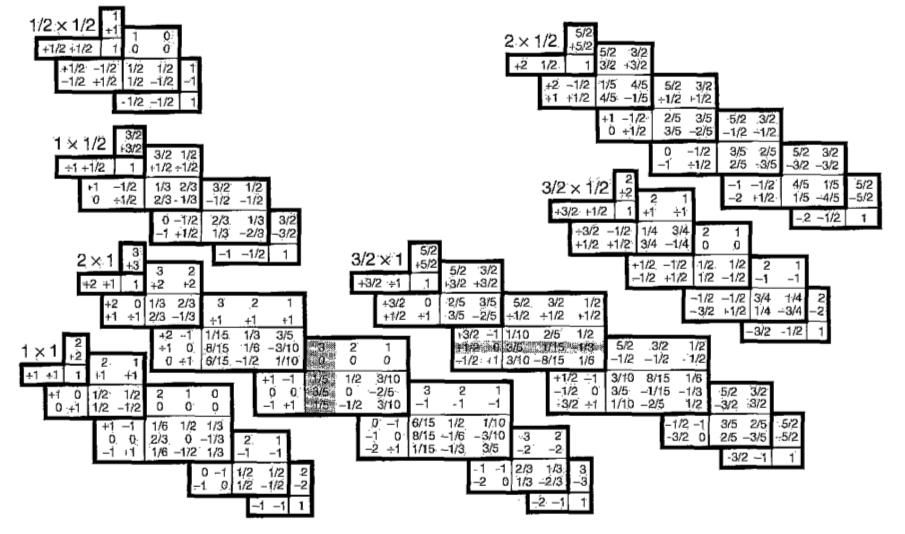
\includegraphics[width=6in]{table}
\caption{The Clebsch-Gordan coefficient table.\cite{griffiths} (A squareroot sign is understood for every entry (see equation \ref{main-model}); The minus sign, if present, goes outside the radical.) In this paper, we only condider the case $J=l+s$. In this case all the coefficients are with positive sign.}
\label{table}
\end{figure*}

The Clebsch-Gordan coefficient table is shown in Figure \ref{table}. According to the table, the coefficients are determined for every set of quantum numbers. The only quantum states whose coefficients can be determined easily are the ones with $J=m_J$, $l=m_l$ and $s=m_s$. Such quantum states are called initial states.

Besides the conditions of quantum states, initial states also satisfy the following conditions:

\begin{enumerate}

\item The initial states have this form: ((1 . ($j$ . $m_j$)) . ((1 . (($l$ . $m_l$) . (s . $m_s$)))))

\item $m_l= l$, $m_s=s$, $m_j = j$

\item There is only one coupled element in the coupled list

\end{enumerate}

Function initial-quantum-state verifies whether the input satisfies the conditions above. It is implemented as follows:

\begin{acl2-lst}
(defun initial-quantum-state (x)
 (and (equal (j-coefficient (get-jstate x)) 1)
  (equal (first-coupled-coefficient 
	  (get-coupled-state x)) 
   1)
  (equal (len (get-coupled-state x)) 1)
  (equal (quantum-j (get-jstate x))
   (quantum-mj (get-jstate x)))
  (equal (first-coupled-l (get-coupled-state x))
   (first-coupled-ml (get-coupled-state x)))
  (equal (first-coupled-s (get-coupled-state x))
   (first-coupled-ms (get-coupled-state x)))
  (true-quantum-state x)))
\end{acl2-lst}

Serveral properties of initial states are proved in ACL2 theorem prover.

\subsection{An Initial State is a Quantum State}

The implementation of this theorem is shown as follows:

\begin{acl2-lst}
(defthm initial-quantum-state-valid 
 (implies (initial-quantum-state x)
  (true-quantum-state x)))
\end{acl2-lst}

\subsection{Normalize Initial States}

Since the coefficient of J-state and the coefficient of the only coupled states are 1, the normalization of initial state is indeed the initial state itself. The implementation of the theorem is shown as follows:

\begin{acl2-lst}
(defthm initial-state-lemma-5
 (implies (initial-quantum-state x)
  (equal (normalize-helper 1 
			(get-coupled-state x))
   (get-coupled-state x))))
\end{acl2-lst}

\subsection{Cleaning up Zeros in Initial States}

Since an initial state does not have elements equal to 0, function clean-up-zero does not change the output of the lowering operators applying on the initial states. The theorems which describe this property is implemented as follows:

\begin{acl2-lst}
(defthm initial-state-lemma-6
 (implies (and (none-zero x)
	   (consp x)
	   (true-coupled-list x))
  (equal (clean-up-zero x) x)))

(defthm initial-state-lemma-10
 (implies (initial-quantum-state x)
  (none-zero 
   (l-lowering-operator-helper (cdr x)))))

(defthm initial-state-lemma-15
 (implies (initial-quantum-state x)
  (none-zero 
   (s-lowering-operator-helper (cdr x)))))
\end{acl2-lst}

Lemma 10 and lemma 15 verifythat the L-lowering operators and S-lowering operators do not give lists with zero-elements. Then those two lemmas and lemma 6 together proves that operators operating on the initial states  will not have 0-elements. As the following theorems shown:

\begin{acl2-lst}
(defthm initial-state-lemma-19 
 (implies (initial-quantum-state x)
  (equal (clean-up-zero-list
	  (l-lowering-operator-helper
	   (get-coupled-state x)))
   (l-lowering-operator-helper 
    (get-coupled-state x)))))

(defthm initial-state-lemma-23 
 (implies (initial-quantum-state x)
  (equal (clean-up-zero-list
	  (s-lowering-operator-helper
	   (get-coupled-state x)))
   (s-lowering-operator-helper 
    (get-coupled-state x))))
\end{acl2-lst}

\subsection{L-lowering Operator and S-lowering Operator on Initial States}

This property is very straightforward. If the input is an initial state, then the outputs of l-lowering-operator and s-lowering-operator are real coupled states. The theorems are implemented below.

\begin{acl2-lst}
(DEFTHM
 INITIAL-STATE-LEMMA-29
 (IMPLIES (INITIAL-QUANTUM-STATE X)
  (TRUE-COUPLED-LIST 
     (L-LOWERING-OPERATOR-HELPER (CDR X)))))

(DEFTHM
 INITIAL-STATE-LEMMA-30
 (IMPLIES (INITIAL-QUANTUM-STATE X)
  (TRUE-COUPLED-LIST 
     (S-LOWERING-OPERATOR-HELPER (CDR X)))))
\end{acl2-lst}

Note that the two theorems above are proved by the ACL2 proof checker. The advantage of proof in this case is that it can avoid unnecessary case splits and incoreect induction schemes. The detailed implementation is shown in initial-quantum-state.lisp.

\section{Main Theorem: Lowering Operators Operating on Initial States}

\subsection{Proof by Hand}

The proof by hand is very straightforward. According to equation \ref{main-model}, we have 

\begin{equation}
|J, m_J \rangle= |l,m_l\rangle |s,m_s\rangle
\label{initial1}
\end{equation} 

Then we apply the J-lowering operator to the left-hand side of equation \ref{initial1}, and L-lowering as well as S-lowering operator on the right-hand side. According to equations \ref{j}, \ref{l} and \ref{s}, we have 

\begin{equation}
\begin{aligned}
\sqrt{2J}|J,m_J -1\rangle = \sqrt{2l} |l,m_l-1\rangle|s,m_s\rangle\\ + \sqrt{2s}|l,m_l\rangle|s,m_s-1\rangle
\end{aligned}
\label{initial2}
\end{equation}

Since $J=l+s$, we can know $2J=2l+2s$. The Clebsch-Gordan coefficients calculated using lowering operators in this case is correct.

\subsection{Proof by ACL2}

The ACL2 theorem is listed below:

\begin{acl2-lst}
(DEFTHM INITIAL-STATE-LOWERING-VALID
 (IMPLIES (INITIAL-QUANTUM-STATE X)
  (TRUE-QUANTUM-STATE 
	(QUANTUM-OPERATOR X))))
\end{acl2-lst}

The implementation of this theorem is in main-theorem-1.lisp. Initially, theorem prover is used to expand and simplify the functions. Then a prove command is used in order to utilize ACL2 power to prove this main theorem. This theorem is successfully proved and hence the application of lowering operators operaing on initial states gives correct Clebsch-Gordan coefficients.

\section{Future Research}

In fact, given an initial state, any number of times the application of the lowering operators on the initial state until the state with invalid quantum numbers (0 . 0) returns a state with correct Clebsch-Gordan coefficients (equation \ref{probability}). The idea is shown as follows:

\begin{acl2-lst}
(skip-proofs
 (defun all-lowering-valid (x)
  (if (equal x (cons '0 '0))
   t
   (and (true-quantum-state 
	 (quantum-operator x))
    (all-lowering-valid 
     (quantum-operator x)))))

(defthm all-quantum-lowering-valid 
	(implies (inital-quantum-state x)
		 (all-lowering-valid x)))

\end{acl2-lst}

Here function all-lowering-valid detemines whether any number of lowering operations on the input until (0 . 0) gives a correct quantum state. Theorem all-quantum-lowering-valid is served as proving the property described above.

However, function all-lowering-valid is not a valid function definition according to \cite{acl2}. Therefore a valid definition is essential. In addition, proving this theorem will need a large number of lemmas due to the fact that equation \ref{merge} is complicated. Those difficulties are need to overcome in the future.

We can also eliminate the restriction that $J=l+s$. Consequently, $J=|l-s|,|l-s|+1,\ldots ,l+s$. There are more cases to consider and the equation of calculating merged coefficient (similar to equation \ref{merge}) will be signifincanly more complicated. Hence, the genralization of lowering operators applying to all quantum states is the ultimate goal.

\section{Conclusion}

This paper provides a detailed description on how to use ACL2 theorem prover to prove the correctness of lowering operators operating on the initial state when $J=l+s$. My model of quantum state consists of a J-state and a list of coupled states. The J-lowering operator operates on J-state while L-lowering and S-lowering operators operate on coupled states. The input and output of lowering operators are of the form shown in equation \ref{main-model}. 

The main theorem of this project is given an initial state, the first application of lowering operators return a quantum state with correct Clebsch-Gordan coefficients. Proving this theorem manually is not complicated. However, the proof of this theorem is a fundamental step on the future research shown in Section 6.

The ultimate goal for this project is to prove the correctness of lowering operators applying to all quantum states. Due to the fact that quantum states have a large number of cases, the number of case splits will be large. Thus special care is necessary in the future research. 

% use section* for acknowledgement
\ifCLASSOPTIONcompsoc
  % The Computer Society usually uses the plural form
  \section*{Acknowledgments}
\else
  % regular IEEE prefers the singular form
  \section*{Acknowledgment}
\fi


The author would like to thank Professor Warren Hunt, Teaching Assistant Nathan Wetzler, Dr. Matthew Kaufmann and Cuong Chau for helping me implementing this project. Their help is very important. I learned significant amount of knowledge from them and I believe such knowledge will be very useful in the future.


% Can use something like this to put references on a page
% by themselves when using endfloat and the captionsoff option.
\ifCLASSOPTIONcaptionsoff
  \newpage
\fi



% trigger a \newpage just before the given reference
% number - used to balance the columns on the last page
% adjust value as needed - may need to be readjusted if
% the document is modified later
%\IEEEtriggeratref{8}
% The "triggered" command can be changed if desired:
%\IEEEtriggercmd{\enlargethispage{-5in}}

% references section

% can use a bibliography generated by BibTeX as a .bbl file
% BibTeX documentation can be easily obtained at:
% http://www.ctan.org/tex-archive/biblio/bibtex/contrib/doc/
% The IEEEtran BibTeX style support page is at:
% http://www.michaelshell.org/tex/ieeetran/bibtex/
\bibliographystyle{IEEEtran}
% argument is your BibTeX string definitions and bibliography database(s)
\bibliography{reference}
%
% <OR> manually copy in the resultant .bbl file
% set second argument of \begin to the number of references
% (used to reserve space for the reference number labels box)

% that's all folks
\end{document}


